\subsection{Exam: 2022. 05. 30., Exercise 3}

\lineparagraph{Exercise}

Consider the following decision problem. We are given an undirected connected
graph $G$ of even number of vertices, whose edges are colored red or blue.
We want to decide whether there exists a Hamiltonian cycle in $G$ that consists
of a red path and a blue path ofthe same length, that is, going along the
Hamiltonian cycle, the red edges form a path and the blue edges form a path
and those two paths have the same number of vertices. Prove that this problem
is NP-complete.

\lineparagraph{Solution}

I belive this exercise caused the most problems and misunderstandings on the exam,
so let's break down and understand what we are being asked for here.

\begin{itemize}
\item We are given decision problem, let's name its language $HAMRB$, for Hamiltonian-cycle, red-blue version.
\item The input is a graph here, which already has its edges colored in for us in red and blue colors. The coloring is given, we cannot modify this. (Many students did try to color the edges.)
\item We are asked the question, whether there is a Hamiltonian-cycle (a cycle that contains all vertices of the graph) in this graph, which ''red edged half'' and a ''blue edged half'', like so:

\begin{center}
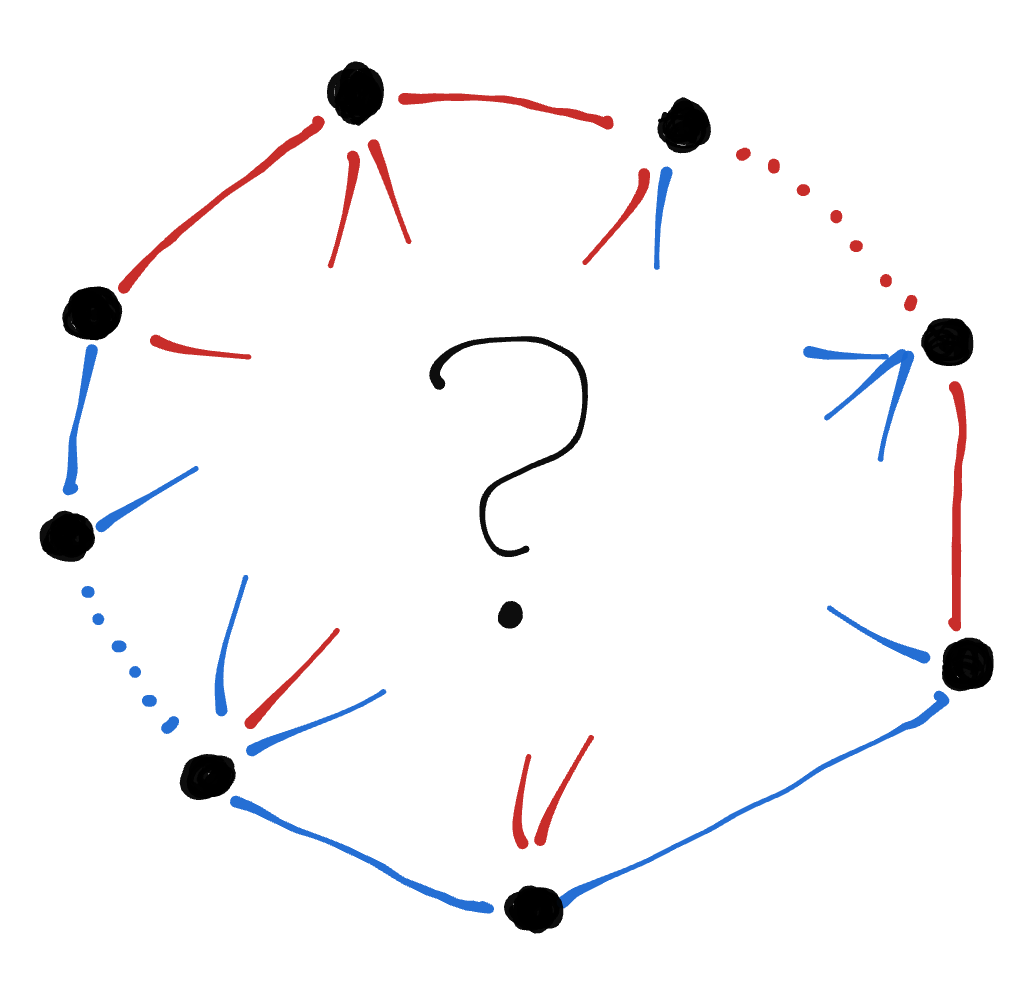
\includegraphics[width=\linewidth]{./exams/2022_05_30/03/hamrb.png}
\end{center}

\end{itemize}